% include the figures path relative to the master file
% \graphicspath{ {./content/method/figures/visual_cues/}{./content/method/figures/}}
\graphicspath{ {./content/method/figures/}}

\section{Materials and Methods}\label{sec:method}
%\todo{Mention texture here, rework where the sections are called}

The proposed method, as well as, its experimental set-up for \ac{oct} volume classification are outlined in Fig.\,\ref{fig:ML-scheme}.
%The methodology is formulated as a standard classification procedure.
The methodology is formulated as a standard classification procedure which consists of five steps.
First, the \ac{oct} volumes are pre-processed as presented in details in Sect.\,\ref{subsec:prepro}.
%Then toward a final descriptor \ac{lbp} and \ac{lbptop} features are extracted with different mapping strategy and represented using two approach.
Then, \ac{lbp} and \ac{lbptop} features are detected, mapped and extracted as discussed in depth in Sect.\,\ref{subsec:feaext}, Sect.\,\ref{subsec:mapping}, and Sect.\,\ref{subsec:fearep}, respectively.
%{\color{red}The feature extraction, mapping, and representation are presented in depth in Sect.\,\ref{subsec:feaext}, Sect.\,\ref{subsec:mapping}, and Sect.\,\ref{subsec:fearep}, respectively. CHECK THE SECTION ORDERING}
Finally, the classification step is presented in Sect.\,\ref{subsec:cls}.


\subsection{Image pre-processing}\label{subsec:prepro}

This section describes the set of pre-processing techniques which aim at enhancing the \ac{oct} volume.
The influence of these pre-processing methods and their possible combinations are extensively studied in Sect.\,\ref{sec:exp}.

\subsubsection{\acf{nlm}}

\begin{figure}[t]
  \centering
  \hspace*{\fill}
  \subfigure[]{\label{subfig:vol}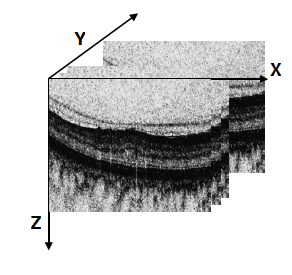
\includegraphics[width=0.3\linewidth]{axs.png}} \hfill
  \subfigure[]{\label{subfig:raw}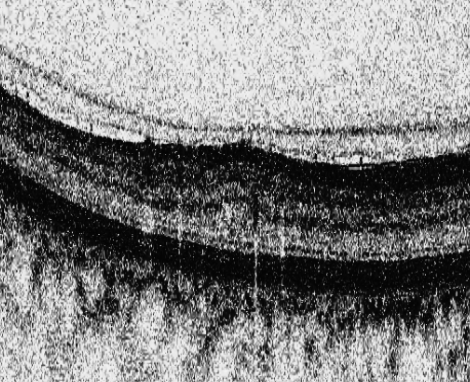
\includegraphics[width=0.3\linewidth]{raw_crop_grey.png}} \hfill
  \subfigure[]{\label{subfig:nlm}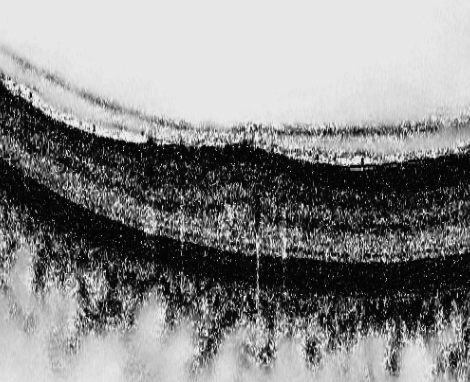
\includegraphics[width=0.3\linewidth]{nlm_crop_grey.png}}
  \hspace*{\fill}
  \caption{\ac{oct}: (a) Organization of the \ac{oct} data - (b) Original image - (c) \ac{nlm} filtering. Note that the images have been negated for visualization purposes.}
  \label{fig:denoise}
\end{figure}


\ac{oct} images suffer from speckle noise, like other image modalities such as \ac{us}~\cite{schmitt1999speckle}.
The \ac{oct} volumes are enhanced by denoising each B-scan (i.e. each $(x$-$z)$ slice) using the \ac{nlm}~\cite{buades2005non}, as shown in Fig.\,\ref{fig:denoise}.
\ac{nlm} has been successfully applied to \ac{us} images to reduce speckle noise and outperforms other common denoising methods~\cite{Coupe2009}.
\ac{nlm} filtering preserves fine structures as well as flat zones, by using all the possible self-predictions that the image can provide rather than local or frequency filters such as Gaussian, anisotropic, or Wiener filters~\cite{buades2005non}.
%An example of filtering using \ac{nlm} filter on \ac{oct} image is depicted in Fig\,\ref{subfig:raw} and Fig.\,\ref{subfig:nlm}.

\subsubsection{Flattening}


\begin{figure}[t]
\centering 
  \hspace*{\fill}
  \subfigure[]{\label{subfig:flatorg}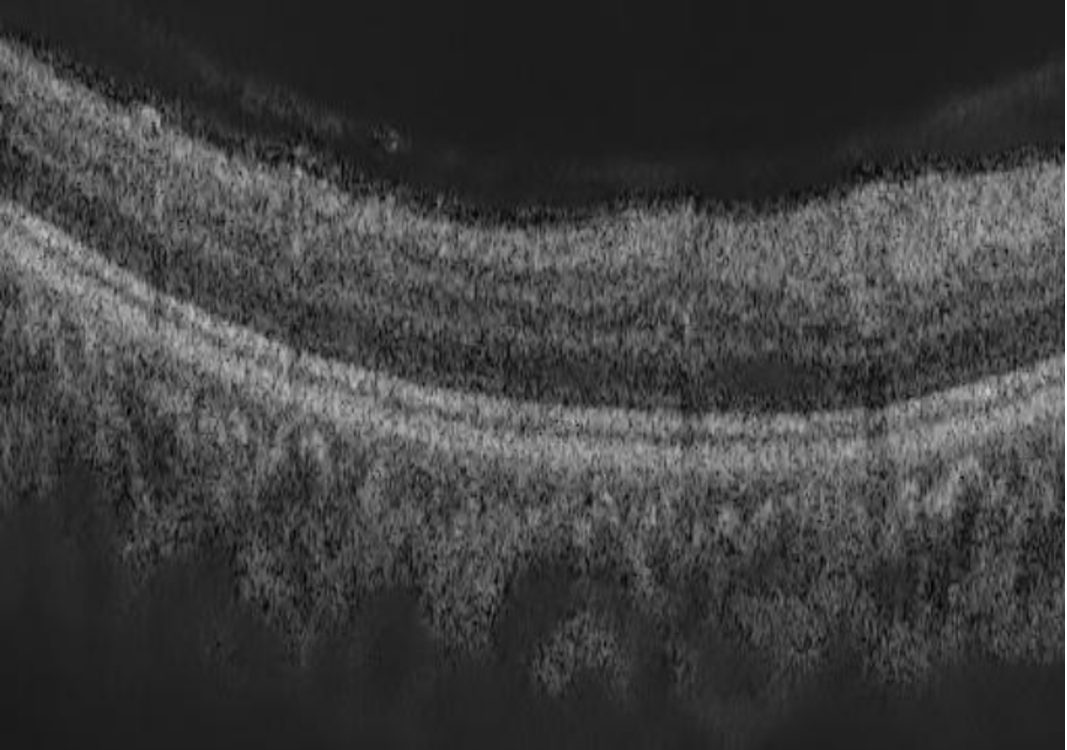
\includegraphics[width=0.20\textwidth]{flattening/original_cropped}}\hfill
  \subfigure[]{\label{subfig:flatotsu}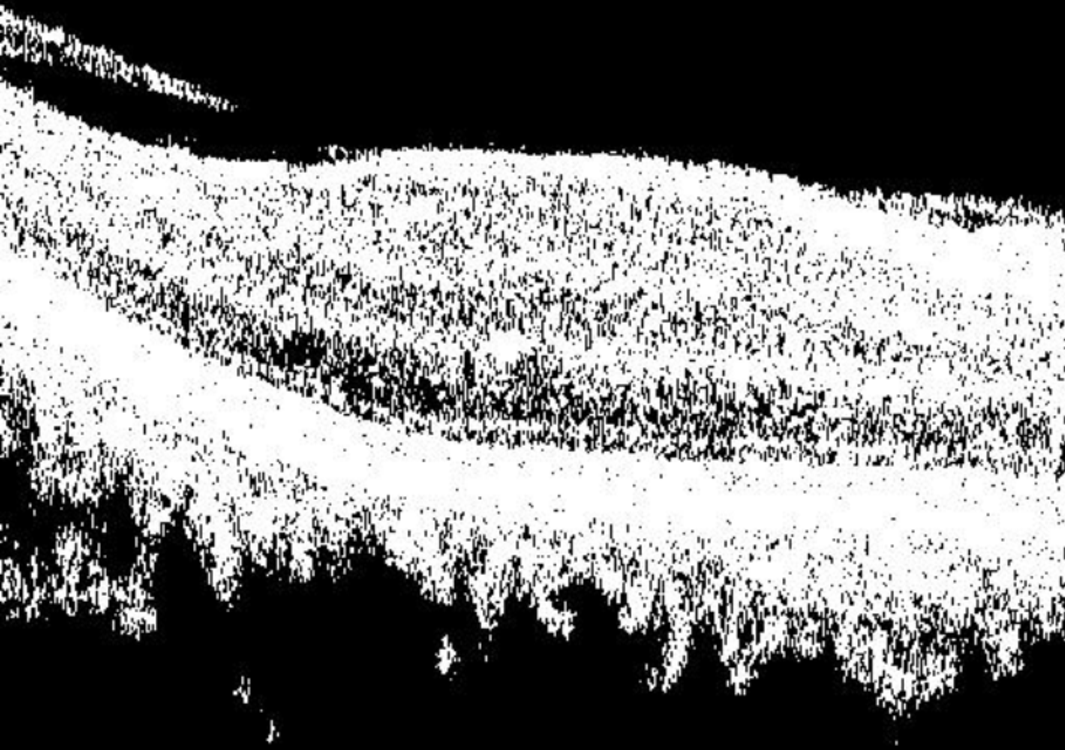
\includegraphics[width=0.20\textwidth]{flattening/thresholding_cropped}}\hfill
  \subfigure[]{\label{subfig:flatmedian}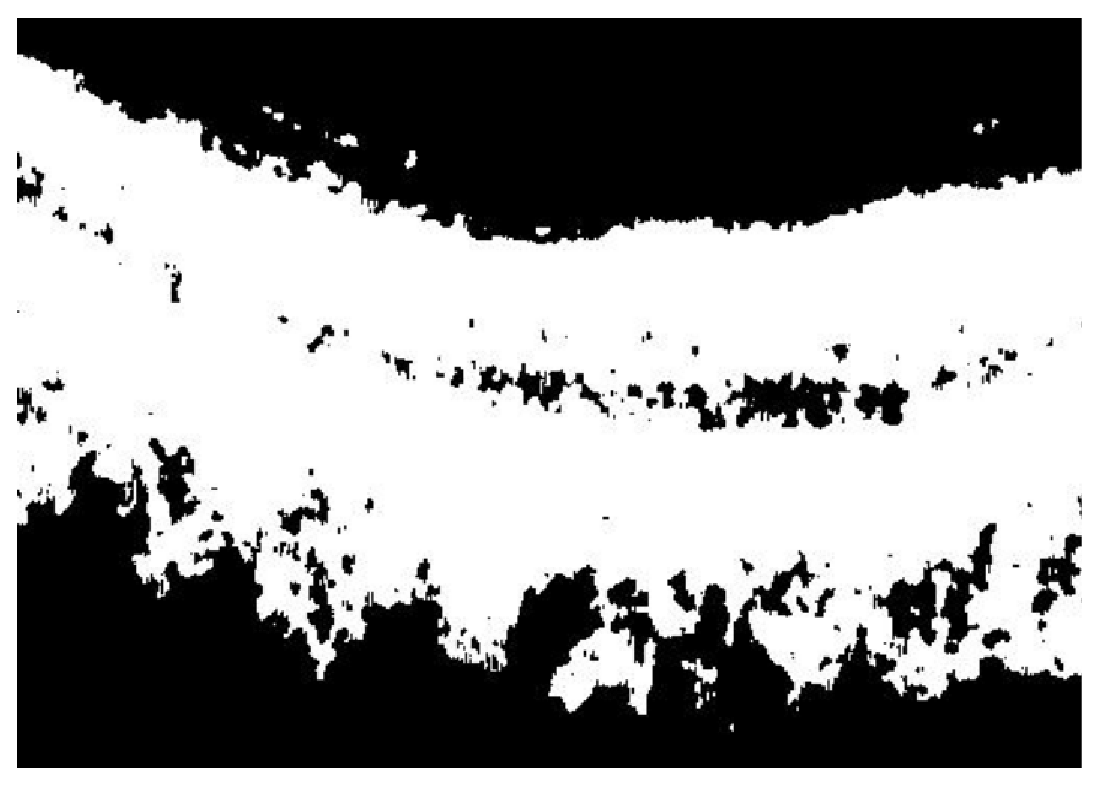
\includegraphics[width=0.20\textwidth]{flattening/median_cropped}}
  \hspace*{\fill}	
  \\
  \hspace*{\fill}
  \subfigure[]{\label{subfig:flatfit}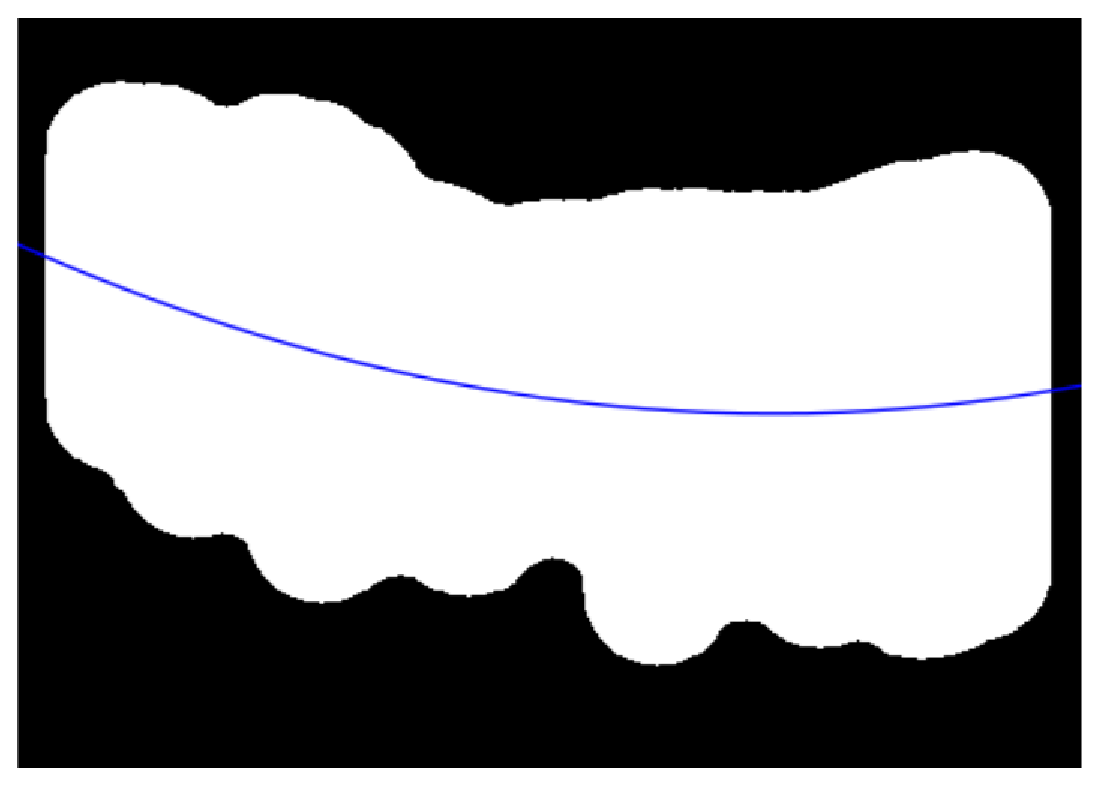
\includegraphics[width=0.20\textwidth]{flattening/fit_cropped}}\hfill
  \subfigure[]{\label{subfig:flatwarp}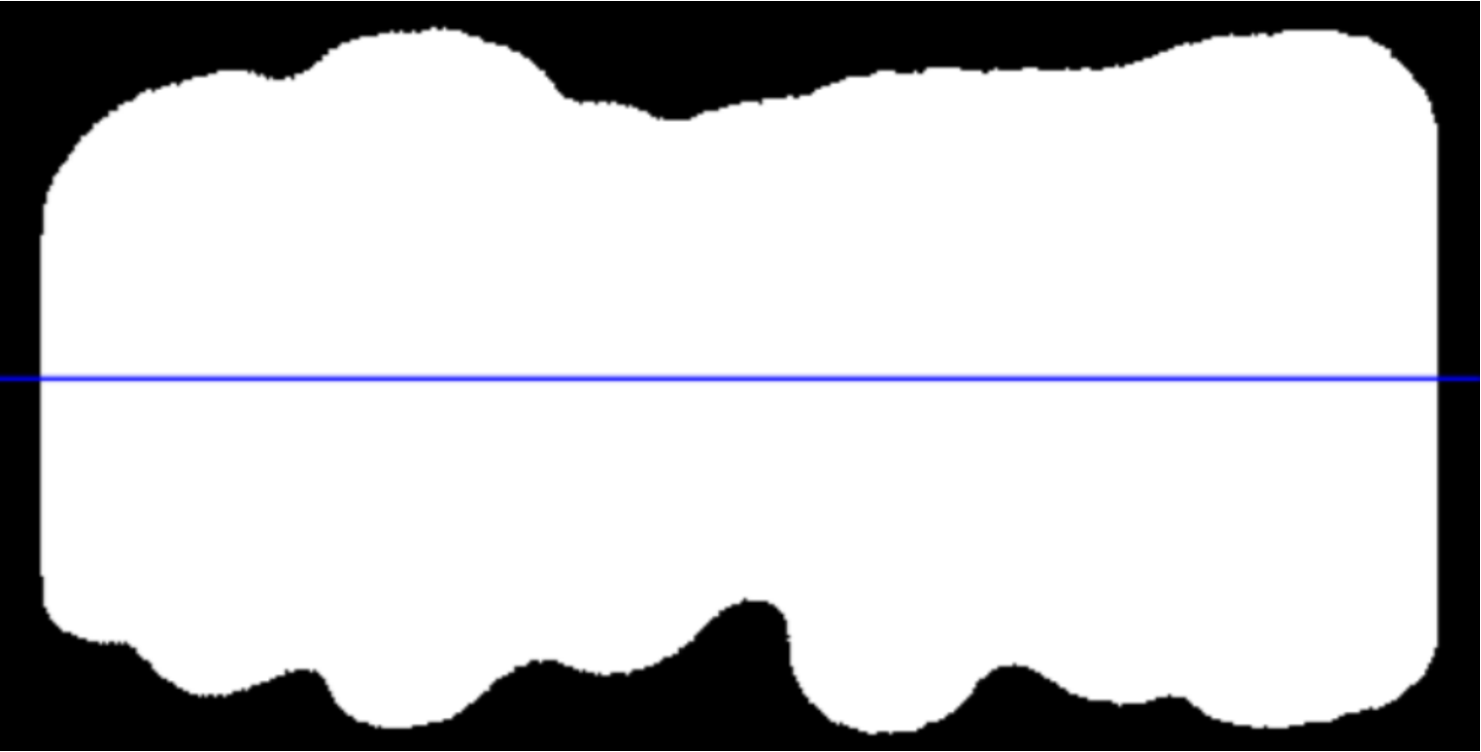
\includegraphics[width=0.20\textwidth]{flattening/warped_cropped}}\hfill
  \subfigure[]{\label{subfig:flatfinal}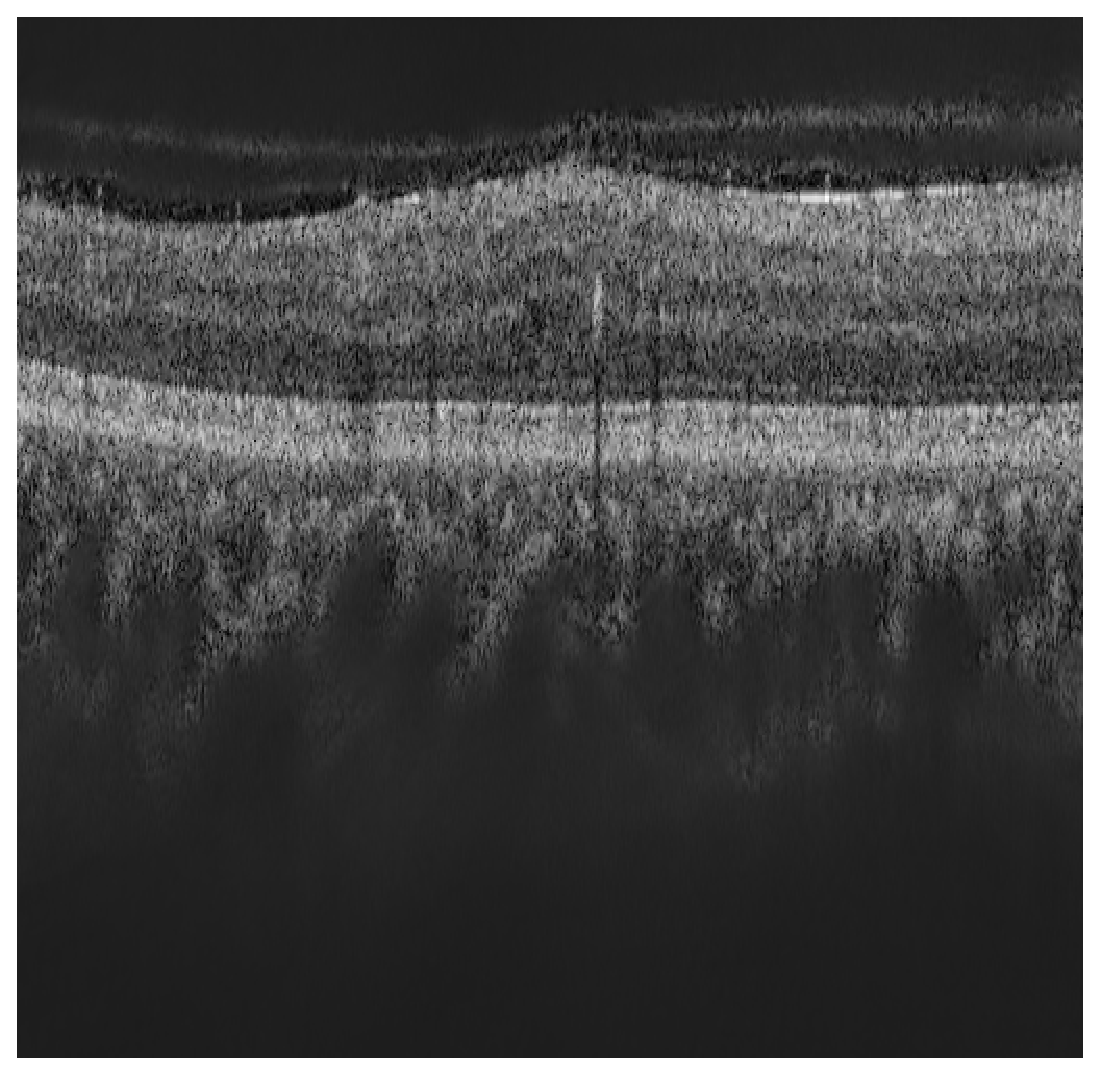
\includegraphics[width=0.20\textwidth]{flattening/warped_org_cropped}}
  \hspace*{\fill}
  \caption{Flattening procedure: (a) original image, (b) thresholding, (c) median filtering, (d) curve fitting, (e) warping, (f) flatten image.}
  \label{fig:flatten}
\end{figure}

Textural descriptors characterize spatial arrangement of intensities.
However, the \ac{oct} scans suffer from large type of variations: inclination angles, positioning, and natural curvature of the retina~\cite{Liu2011}.
Therefore, these variations have to be taken into account to ensure a consistent characterization of the tissue disposition, regardless of the location in the retina.
This invariance can be achieved from different manners: (i) using a rotation invariant descriptor (cf. Sect.\,\ref{subsec:feaext}), or (ii) by unfolding the curvature of the retina.
This latter correction is known as image flattening which theoretically consists of two distinct steps: (i) estimate and fit the curvature of the \ac{rpe} and (ii) warp the \ac{oct} volume such that the \ac{rpe} becomes flat.

Our correction is similar to the one of Liu\,\textit{et al.}~\cite{Liu2011}: each B-scan is thresholded using Otsu's method followed by a median filtering to detect the different retina layers (see Fig\,\ref{subfig:flatmedian} and Fig\,\ref{subfig:flatotsu}). 
Then, a morphological closing and opening is applied to fill the holes and the resulting area is fitted using a second-order polynomial (see Fig.\,\ref{subfig:flatfit}). 
Finally, the scan is warped such that the curve becomes a line as presented in Fig.\,\ref{subfig:flatwarp} and Fig.\,\ref{subfig:flatfinal}. 

%This process of unfolding the curvature of the retina is known as image flattening. When flattening, an estimation of the \rpe  layer is used to modify the volume by imposing that the \rpe  should be flat.
%Our implementation modifies the proposal of Liu\,\textit{et al.}~\cite{Liu2011}, as illustrated in \Cref{fig:flatten}. Othsu thresholding is used to segment the retina from the background. A line is fitted to the bottom part of the segmentation hull, since it is assumed to be parallel to the \rpe. The image is corrected based on this line.

\subsubsection{Slice alignment}
The flattening correction does not enforce an alignment through the \ac{oct} volume.
Thus, in addition to the flattening correction, the warped curves of each B-scan are positioned at the same altitude in the $z$ axis. 

%Similarly, when using 3D texture, misalignment between the slice introduce error to the texture descriptor. In this case the slices are also aligned based on the segmentation's hull.

%\subsubsection{Background cropping}
%\todo[inline]{Cropping out the background allows for less texture to be encoded}

\subsection{Feature detection}\label{subsec:feaext}
In this research, we choose to detect simple and efficient \ac{lbp} texture features with regards to each \ac{oct} slice and volume.
\ac{lbp} is a texture descriptor based on the signs of the differences of a central pixel with respect to its neighboring pixels~\cite{ojala2002multiresolution}.
These differences are encoded in terms of binary patterns as in~Eq.\,\eqref{Eq:LBP}:

\begin{equation}\label{Eq:LBP}
LBP_{P,R} = \sum_{p=0}^{P-1}s(g_{p} - g_{c})2^{p} \ , \qquad s(x) = \begin{cases}
    1  & \ \text{if } x \geq 0\\
    0  & \ \text{otherwise}\\
  \end{cases} \ ,
\end{equation}

\noindent where $g_c$, $g_{p}$ are the intensities of the central pixel and a given neighbor pixel, respectively; $P$ is the number of sampling points in the circle of radius $R$.

Ojala\,\textit{et al.} further extended the original \ac{lbp} formulation to achieve rotation invariance at the expense of limiting the texture description to the notion of circular ``uniformity''~\cite{ojala2002multiresolution}.
Referring to the coordinate system defined in Fig.\,\ref{subfig:vol}, the \ac{lbp} codes are computed on each $(x$-$z)$ slice, leading to a set of \ac{lbp} maps, a map for each $(x$-$z)$ slice.

Volume encoding is later proposed by Zhao\,\textit{et al.} by computing \ac{lbp} descriptors in three orthogonal planes, so called \ac{lbptop}~\cite{zhao2012rotation}.
More precisely, the \ac{lbp} codes are computed considering the $(x$-$z)$ plane, $(x$-$y)$ plane, and $(y$-$z)$ plane, independently.
Thus, three sets of \ac{lbp} maps are obtained, one for each orthogonal plane.

In this research, we consider rotation invariant and uniform \ac{lbp} and \ac{lbptop} features with various sampling points (i.e., $\{8,16,24\}$) with respect to different radius, (i.e., $\{1,2,3\}$).
The number of patterns ($LBP_{\#pat}$) in regards with each configuration is reported in Table~\ref{tab:lbphist}.

%Table.~\ref{tab:lbphist} shows the length of uniform rotation invariant histogram ($\ac{lbp}_{hist}$) for the used sampling point and radius.
\begin{table}
\caption{Number of patterns ($LBP_{\#pat}$) for different sampling points and radius ($\{P,R\}$) of the \ac{lbp} descriptor.}
\centering{
\resizebox{0.5\linewidth}{!}{
\footnotesize{
\begin{tabular}{l  c c c }
\toprule
 \multicolumn{4}{c}{Sampling point for a radius ($\{P, R\}$)}\\
 \midrule
 & $\{8, 1\}$ & $\{16, 2\}$ & $\{24, 3\}$\\
 \cmidrule{2-4}
  $LBP_{\#pat}$  & 10 & 18 & 26 \\
 \bottomrule
\end{tabular}}}}
\label{tab:lbphist}
\end{table}
%\begin{figure}[t]
%  \centering
%  \hspace*{\fill}
%  \subfigure[]{\label{subfig:lbp}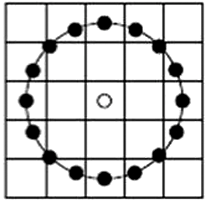
\includegraphics[height=0.1\textheight]{lbp.png}} \hfill
%  \subfigure[]{\label{subfig:lbptop}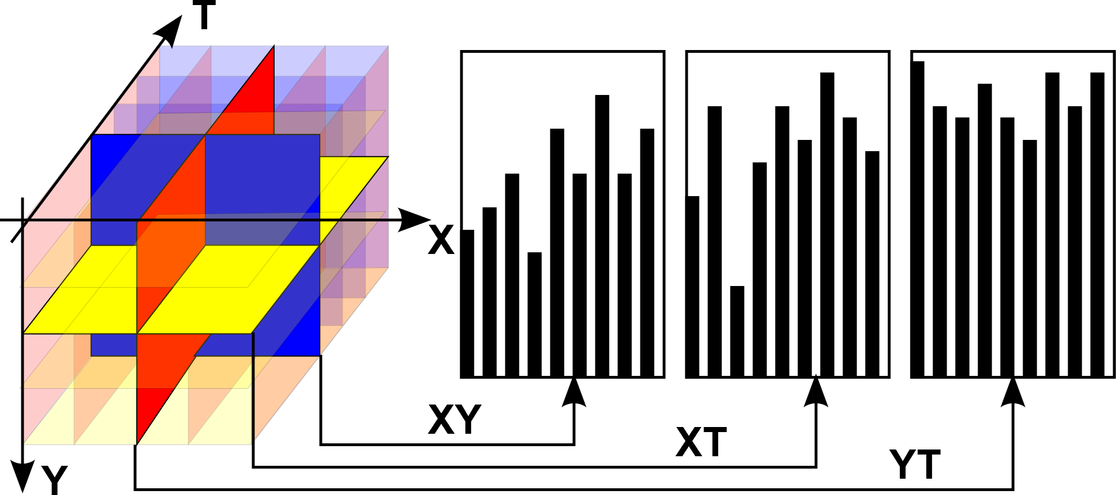
\includegraphics[height=0.1\textheight]{LBPTOP_fig.png}}
%  \hspace*{\fill}
%  \caption{The different \ac{lbp} descriptors: (a) \ac{lbp} with $(R=2,P=16)$ - (b) \ac{lbptop}~\cite{zhao2012rotation}.}
%  \label{fig:lbp}
%\end{figure}

\subsection{Mapping} \label{subsec:mapping}
The mapping stage is used to partition the previously computed \ac{lbp} maps to later extract the final descriptor as presented in the next section.
%The mapping stage is used to determine a discrete set of elements (or structures) which is used for representing the \ac{oct} volume.
For this work, two mapping strategies are defined: (i) \emph{global} and (ii) \emph{local} mapping.

% \begin{figure}[t]
% \begin{center}
% \hspace*{\fill}
% \subfigure[]{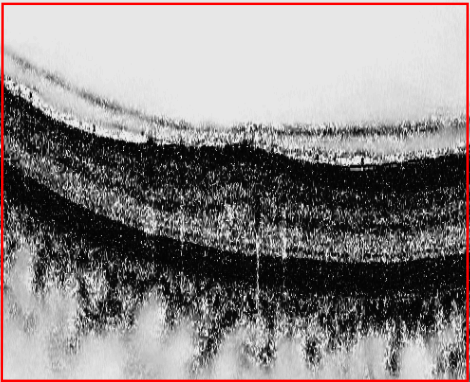
\includegraphics[width=0.22\textwidth]{/mapping/global-2d.png}\label{fig:gm1}}\hfill
% \subfigure[]{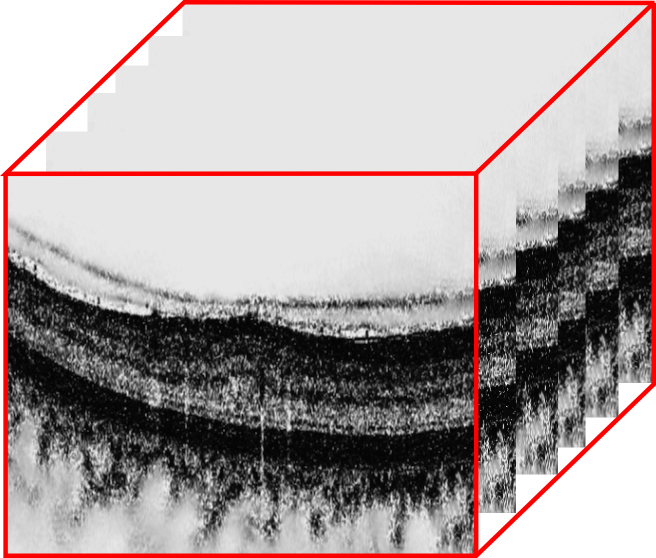
\includegraphics[width=0.22\textwidth]{/mapping/global-3d.png}\label{fig:gm2}}\hfill
% \subfigure[]{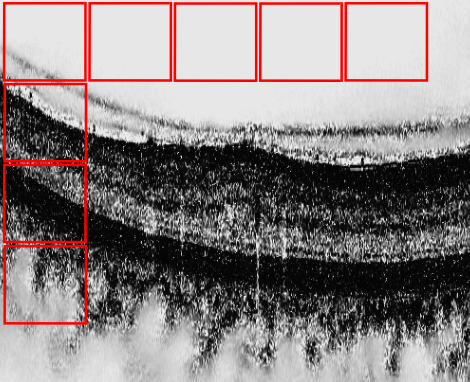
\includegraphics[width=0.22\textwidth]{/mapping/local-2d.png}\label{fig:lm1}}\hfill
% \subfigure[]{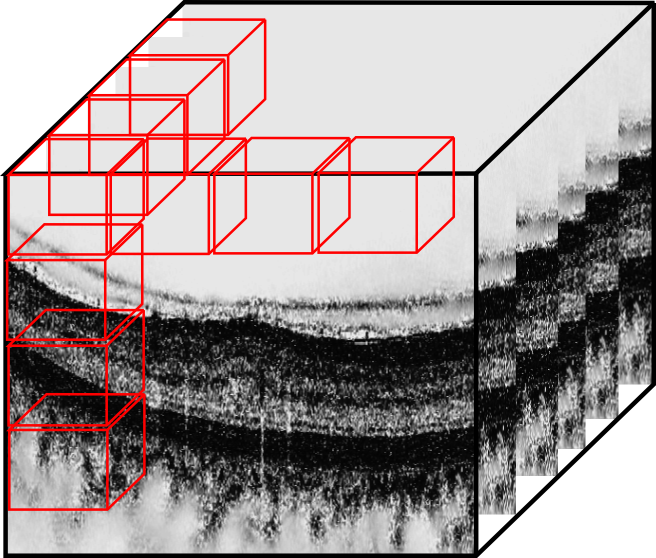
\includegraphics[width=0.22\textwidth]{/mapping/local-3d.png}\label{fig:lm2}}
% \hspace*{\fill}
% \caption{\emph{Global} (a)-(b) and \emph{local} (c)-(d) mapping for \ac{lbp} and \ac{lbptop} features (2D B-scan and 3D volume, respectively).}
% \end{center}
% \label{fig:lgmapping}
% \end{figure}

\begin{table}
\caption{Size of a descriptor for an \ac{sdoct} volume. $d$ denotes the number of slices in the volume, $N$ the number of 2D windows, and $N'$ the number of 3D sub-volumes, respectively.}
\centering{
\footnotesize{
\begin{tabular}{l c c }
  \ctoprule{2-3}
  & Global mapping & Local mapping \\
  \midrule
  \ac{lbp} & $d \times LBP_{\#pat}$ & $(N \times d) \times LBP_{\#pat}$ \\
  \midrule
  \ac{lbptop} & $1 \times (3 \times LBP_{\#pat})$ & $N' \times (3 \times LBP_{\#pat})$ \\
  \bottomrule
\end{tabular}}}
\label{tab:descsize}
\end{table}

\begin{figure}[t]
  \centering
  \hspace*{\fill}
  \subfigure[]{\label{subfig:glbp}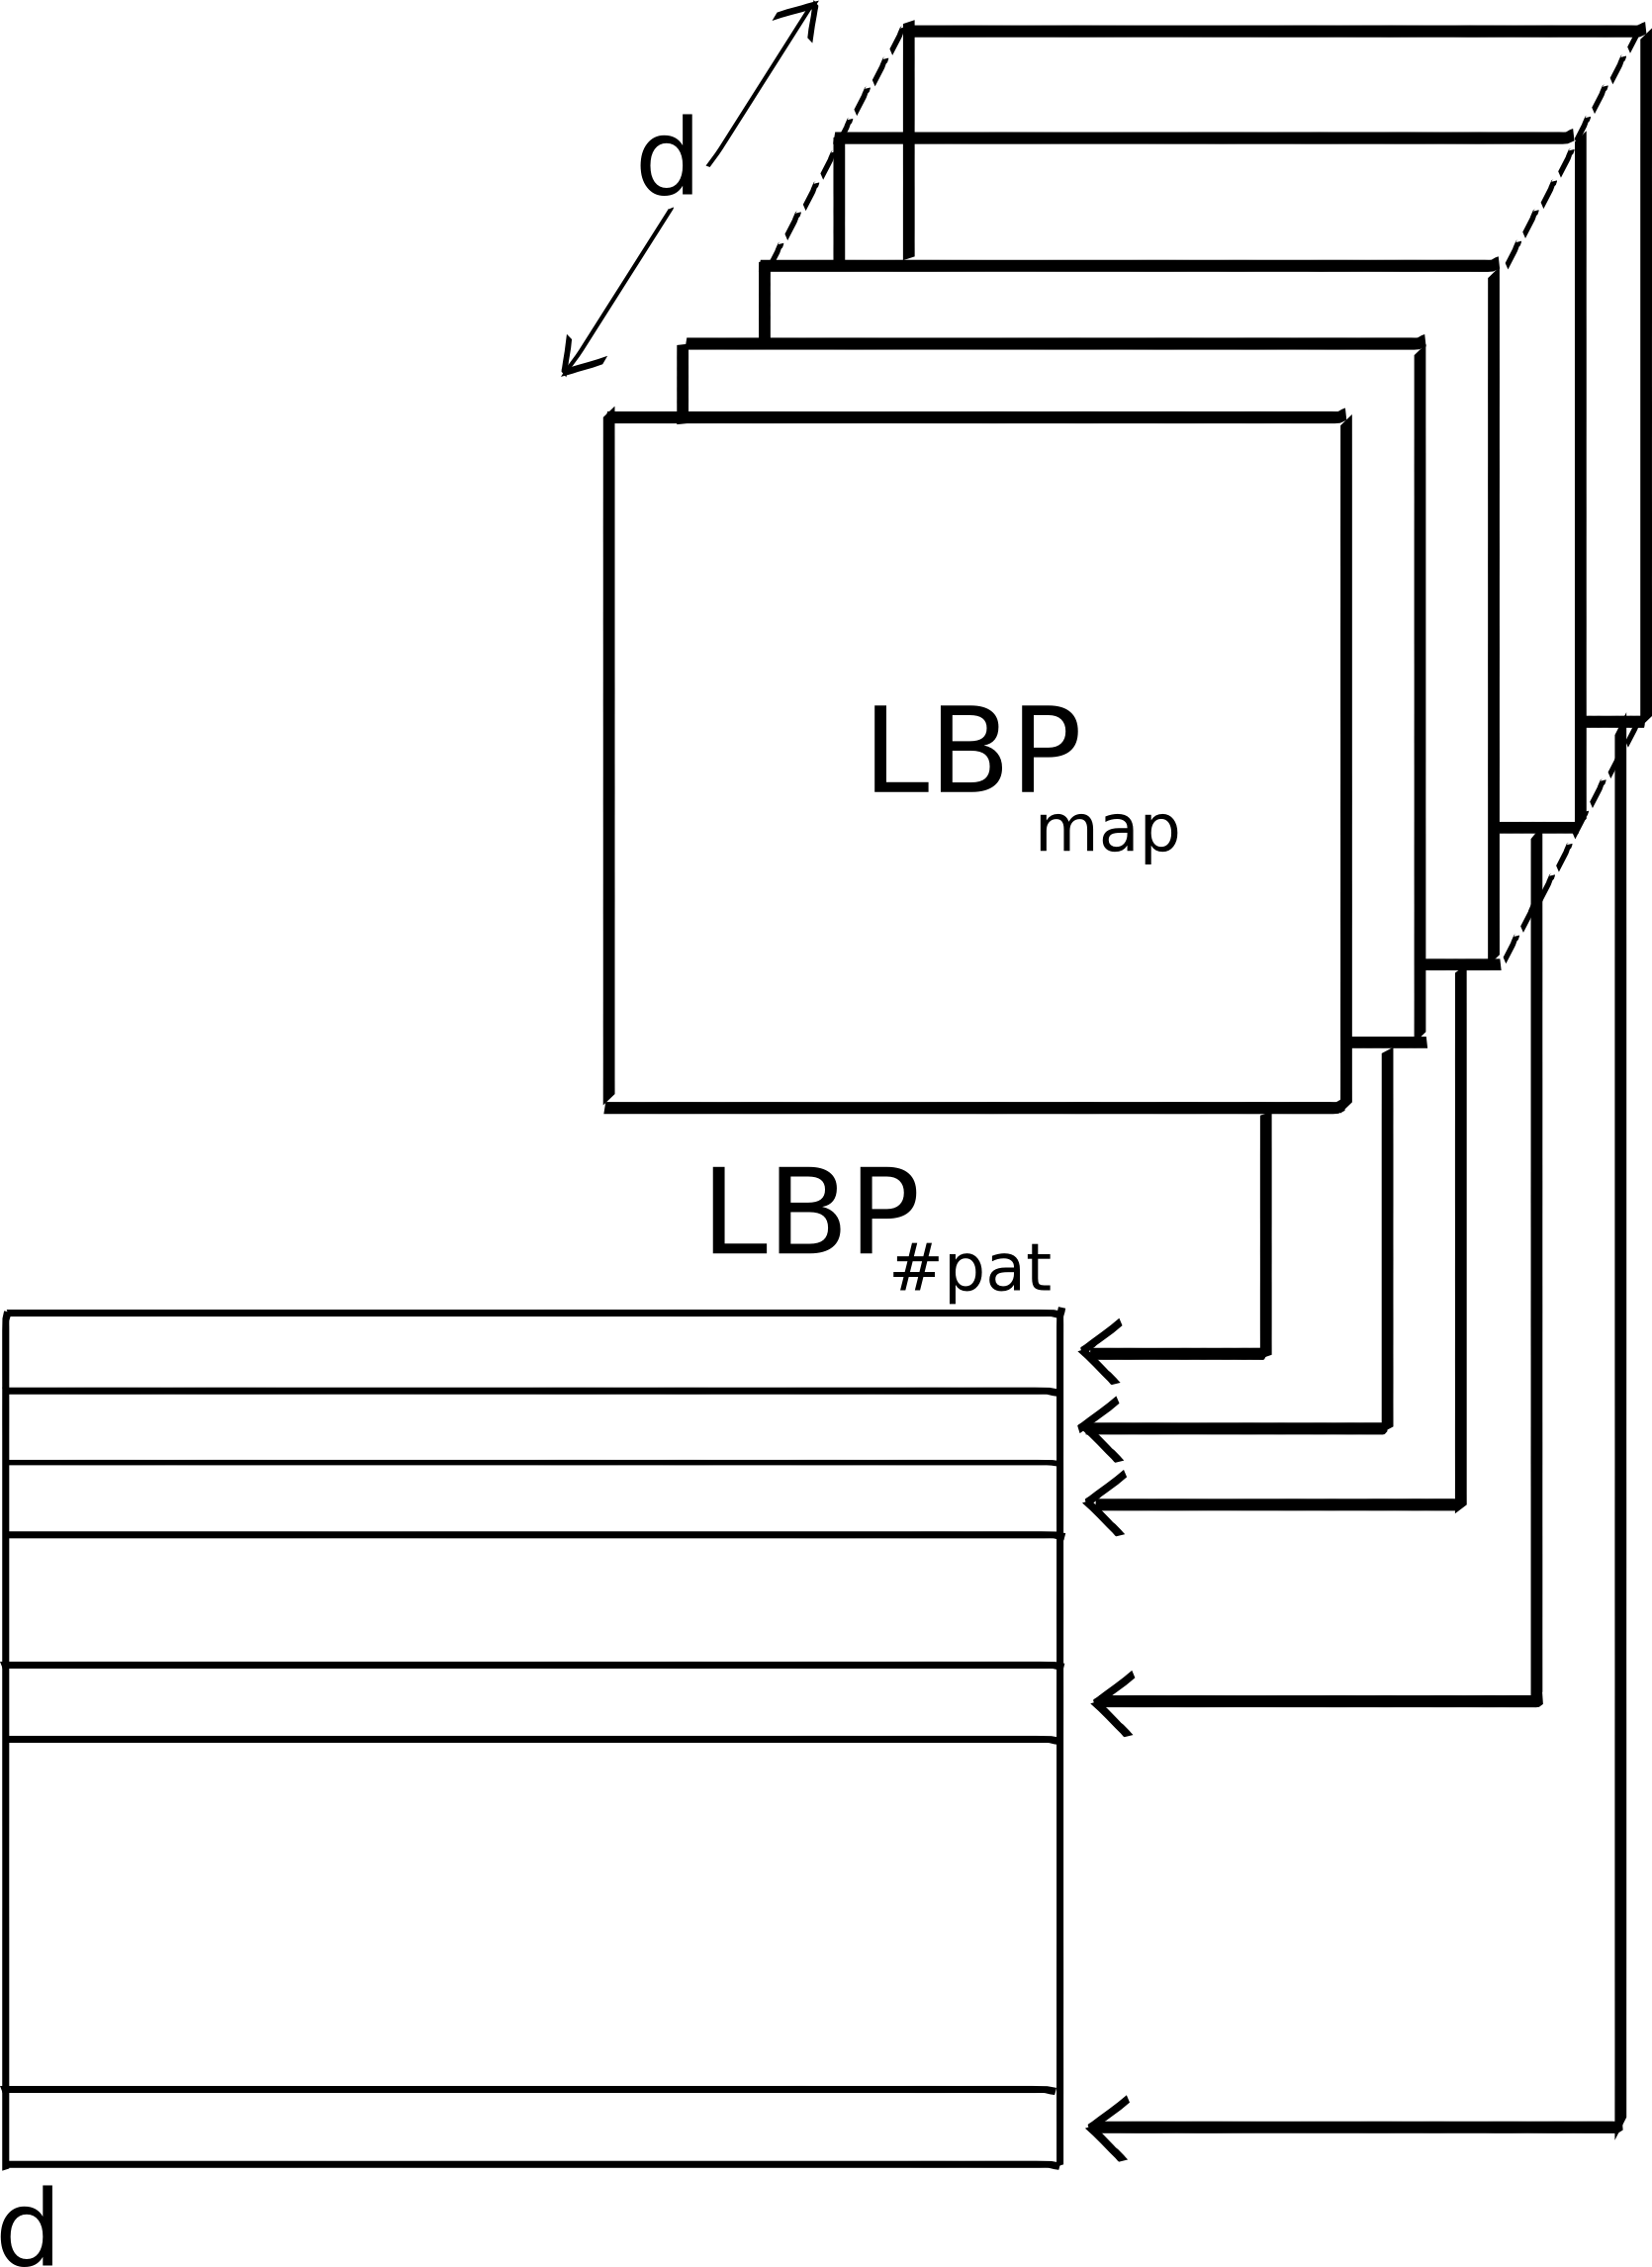
\includegraphics[width=0.25\linewidth]{global-lbp.png}} \hfill
  \subfigure[]{\label{subfig:glbptop}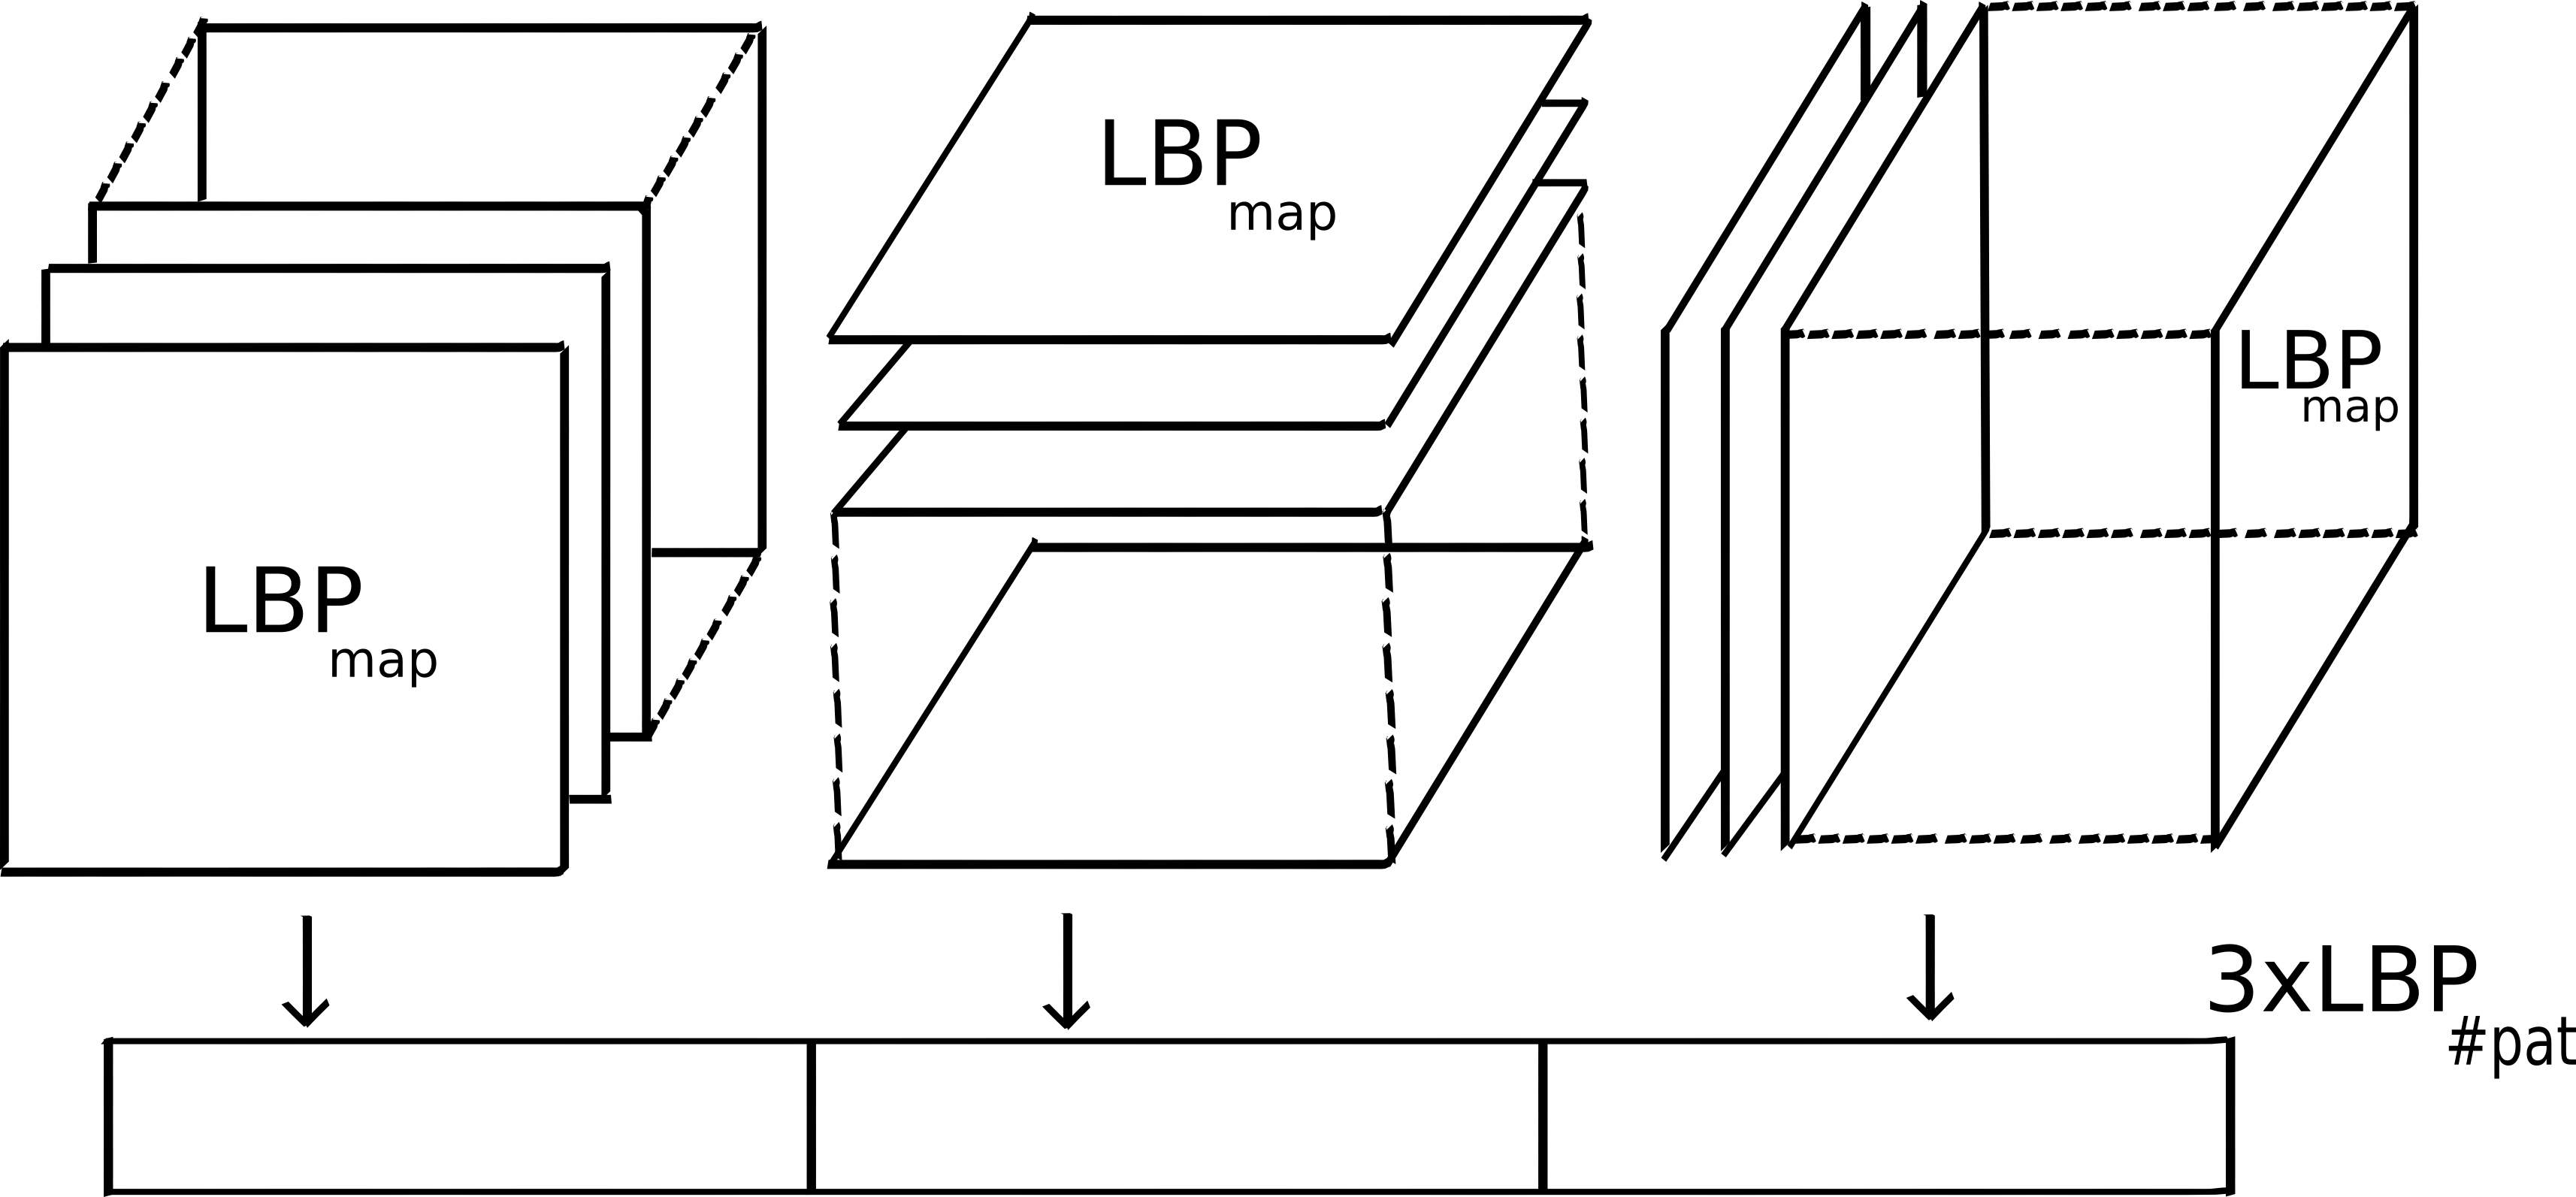
\includegraphics[width=0.48\linewidth]{global-lbptop.png}}
  \hspace*{\fill}\\
  \hspace*{\fill}
  \subfigure[]{\label{subfig:llbp}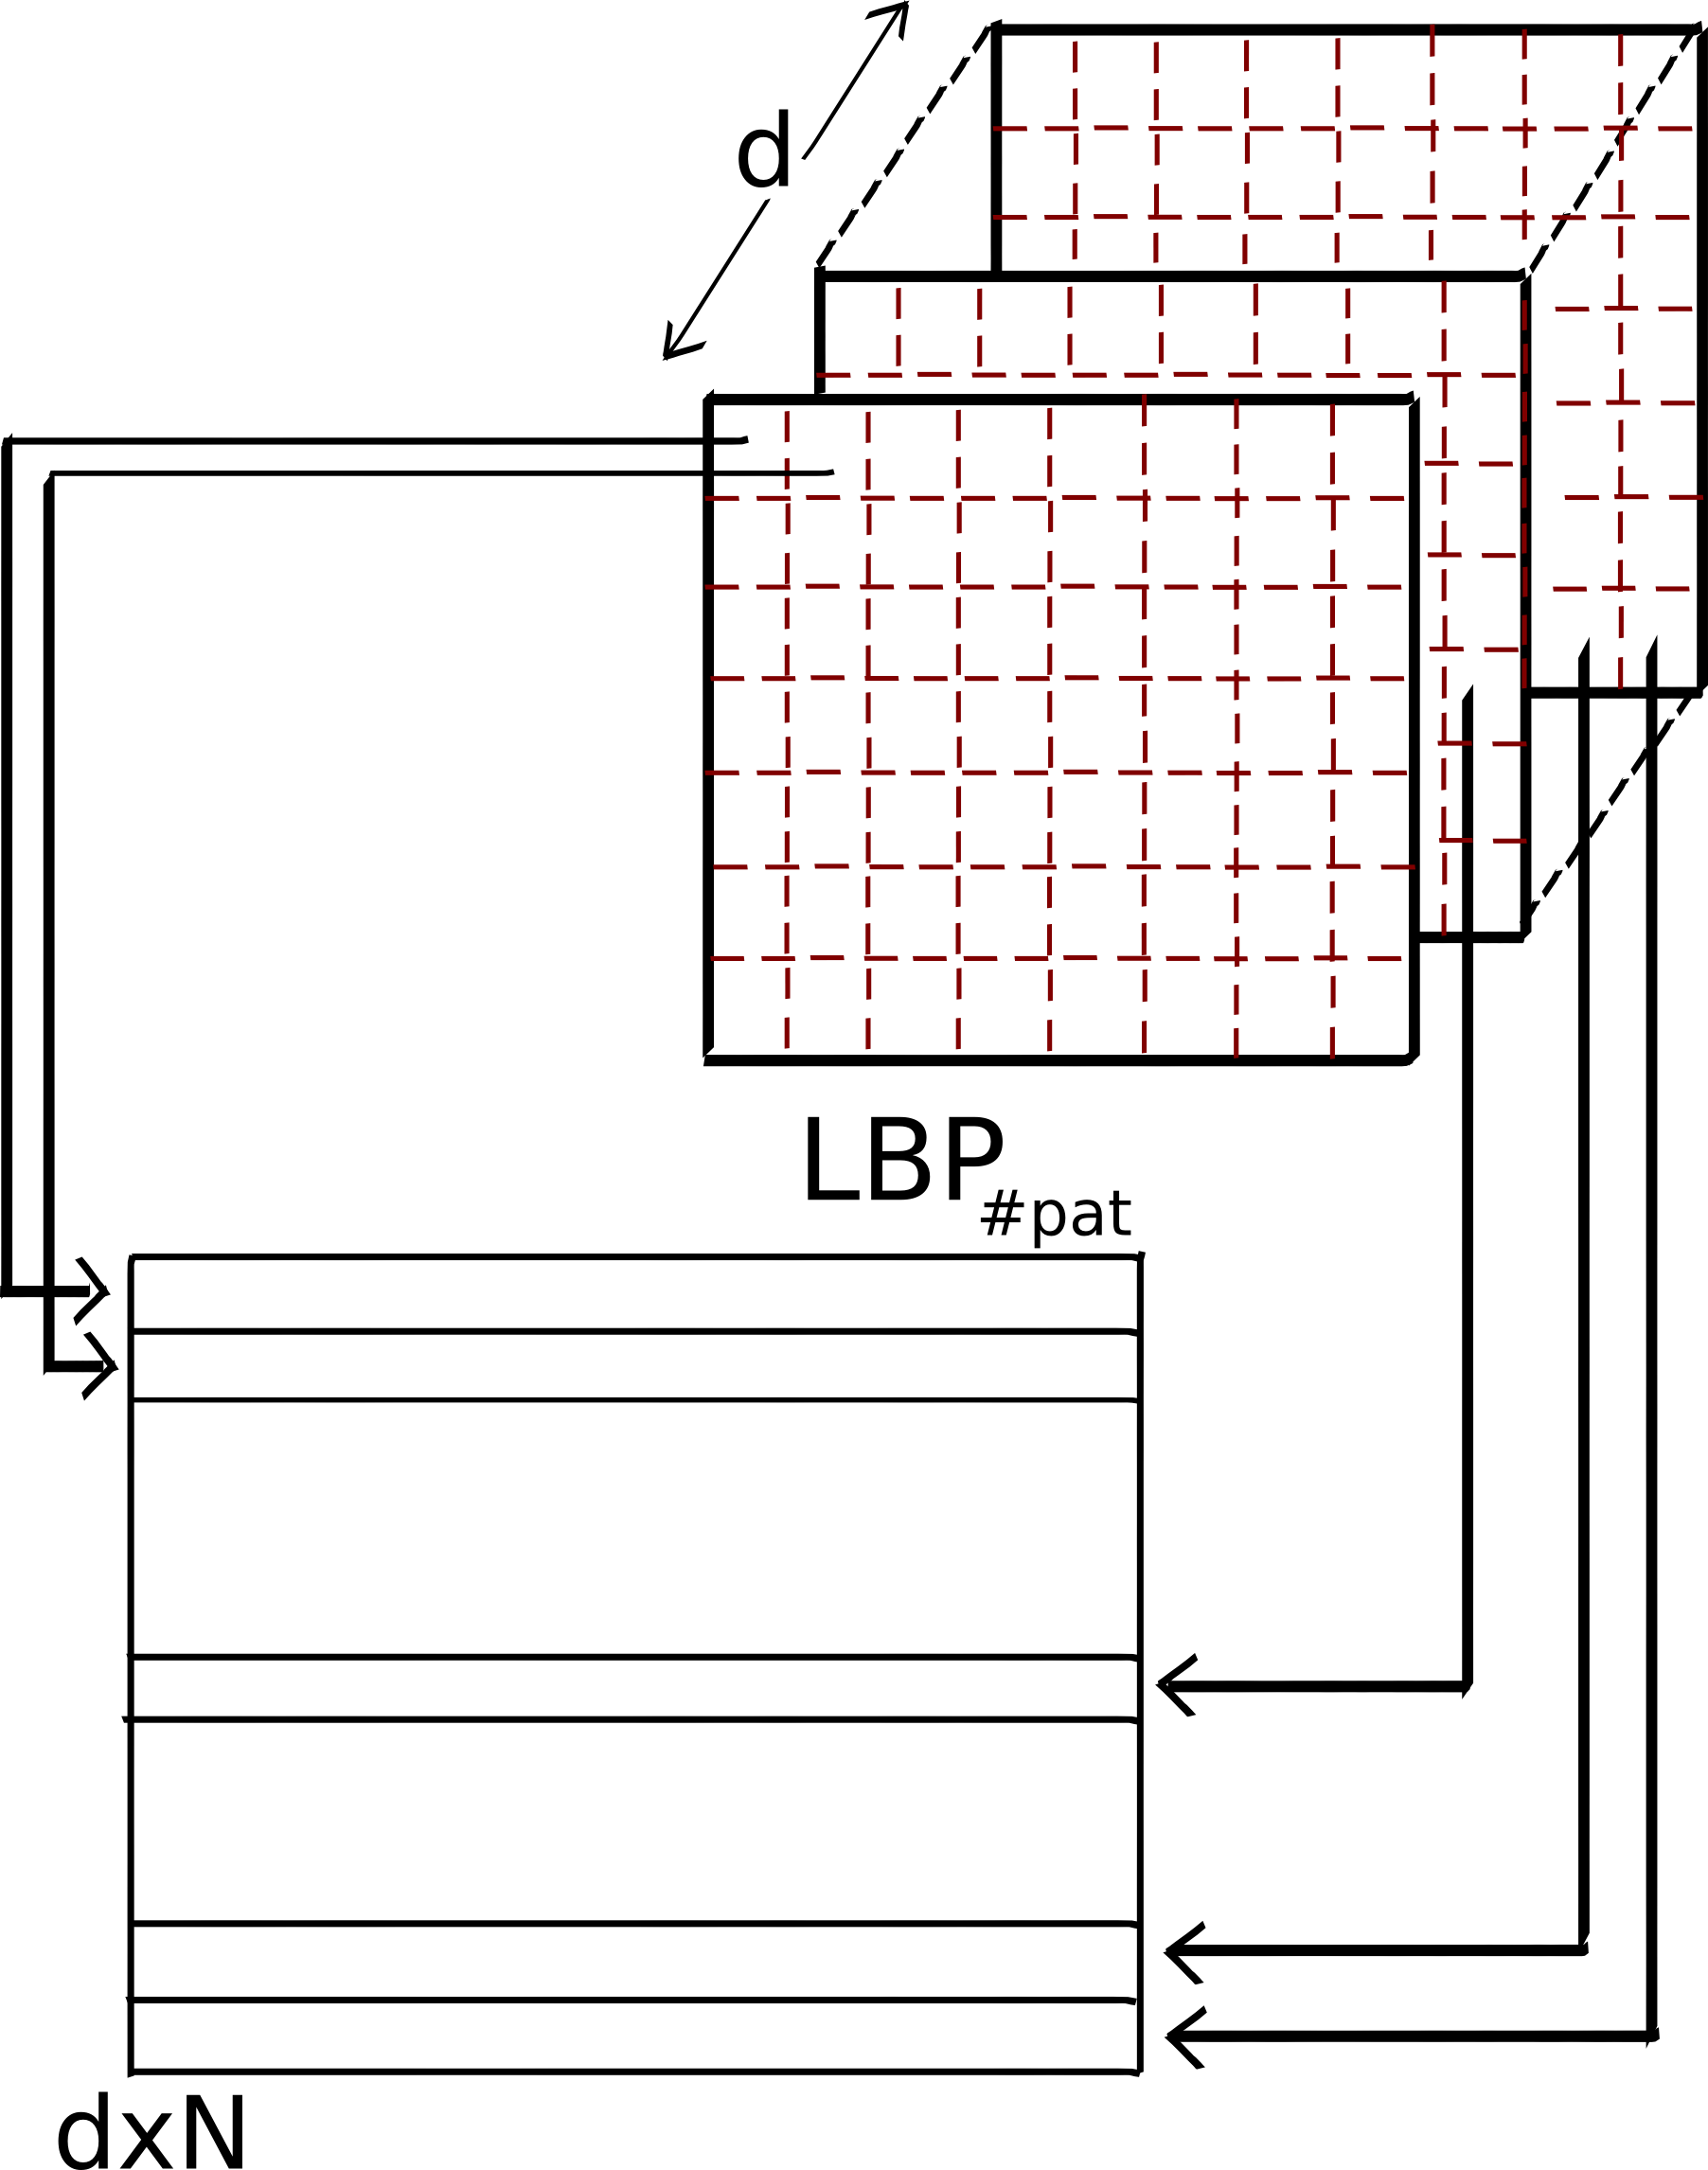
\includegraphics[width=0.25\linewidth]{local-lbp.png}} \hfill
  \subfigure[]{\label{subfig:llbptop}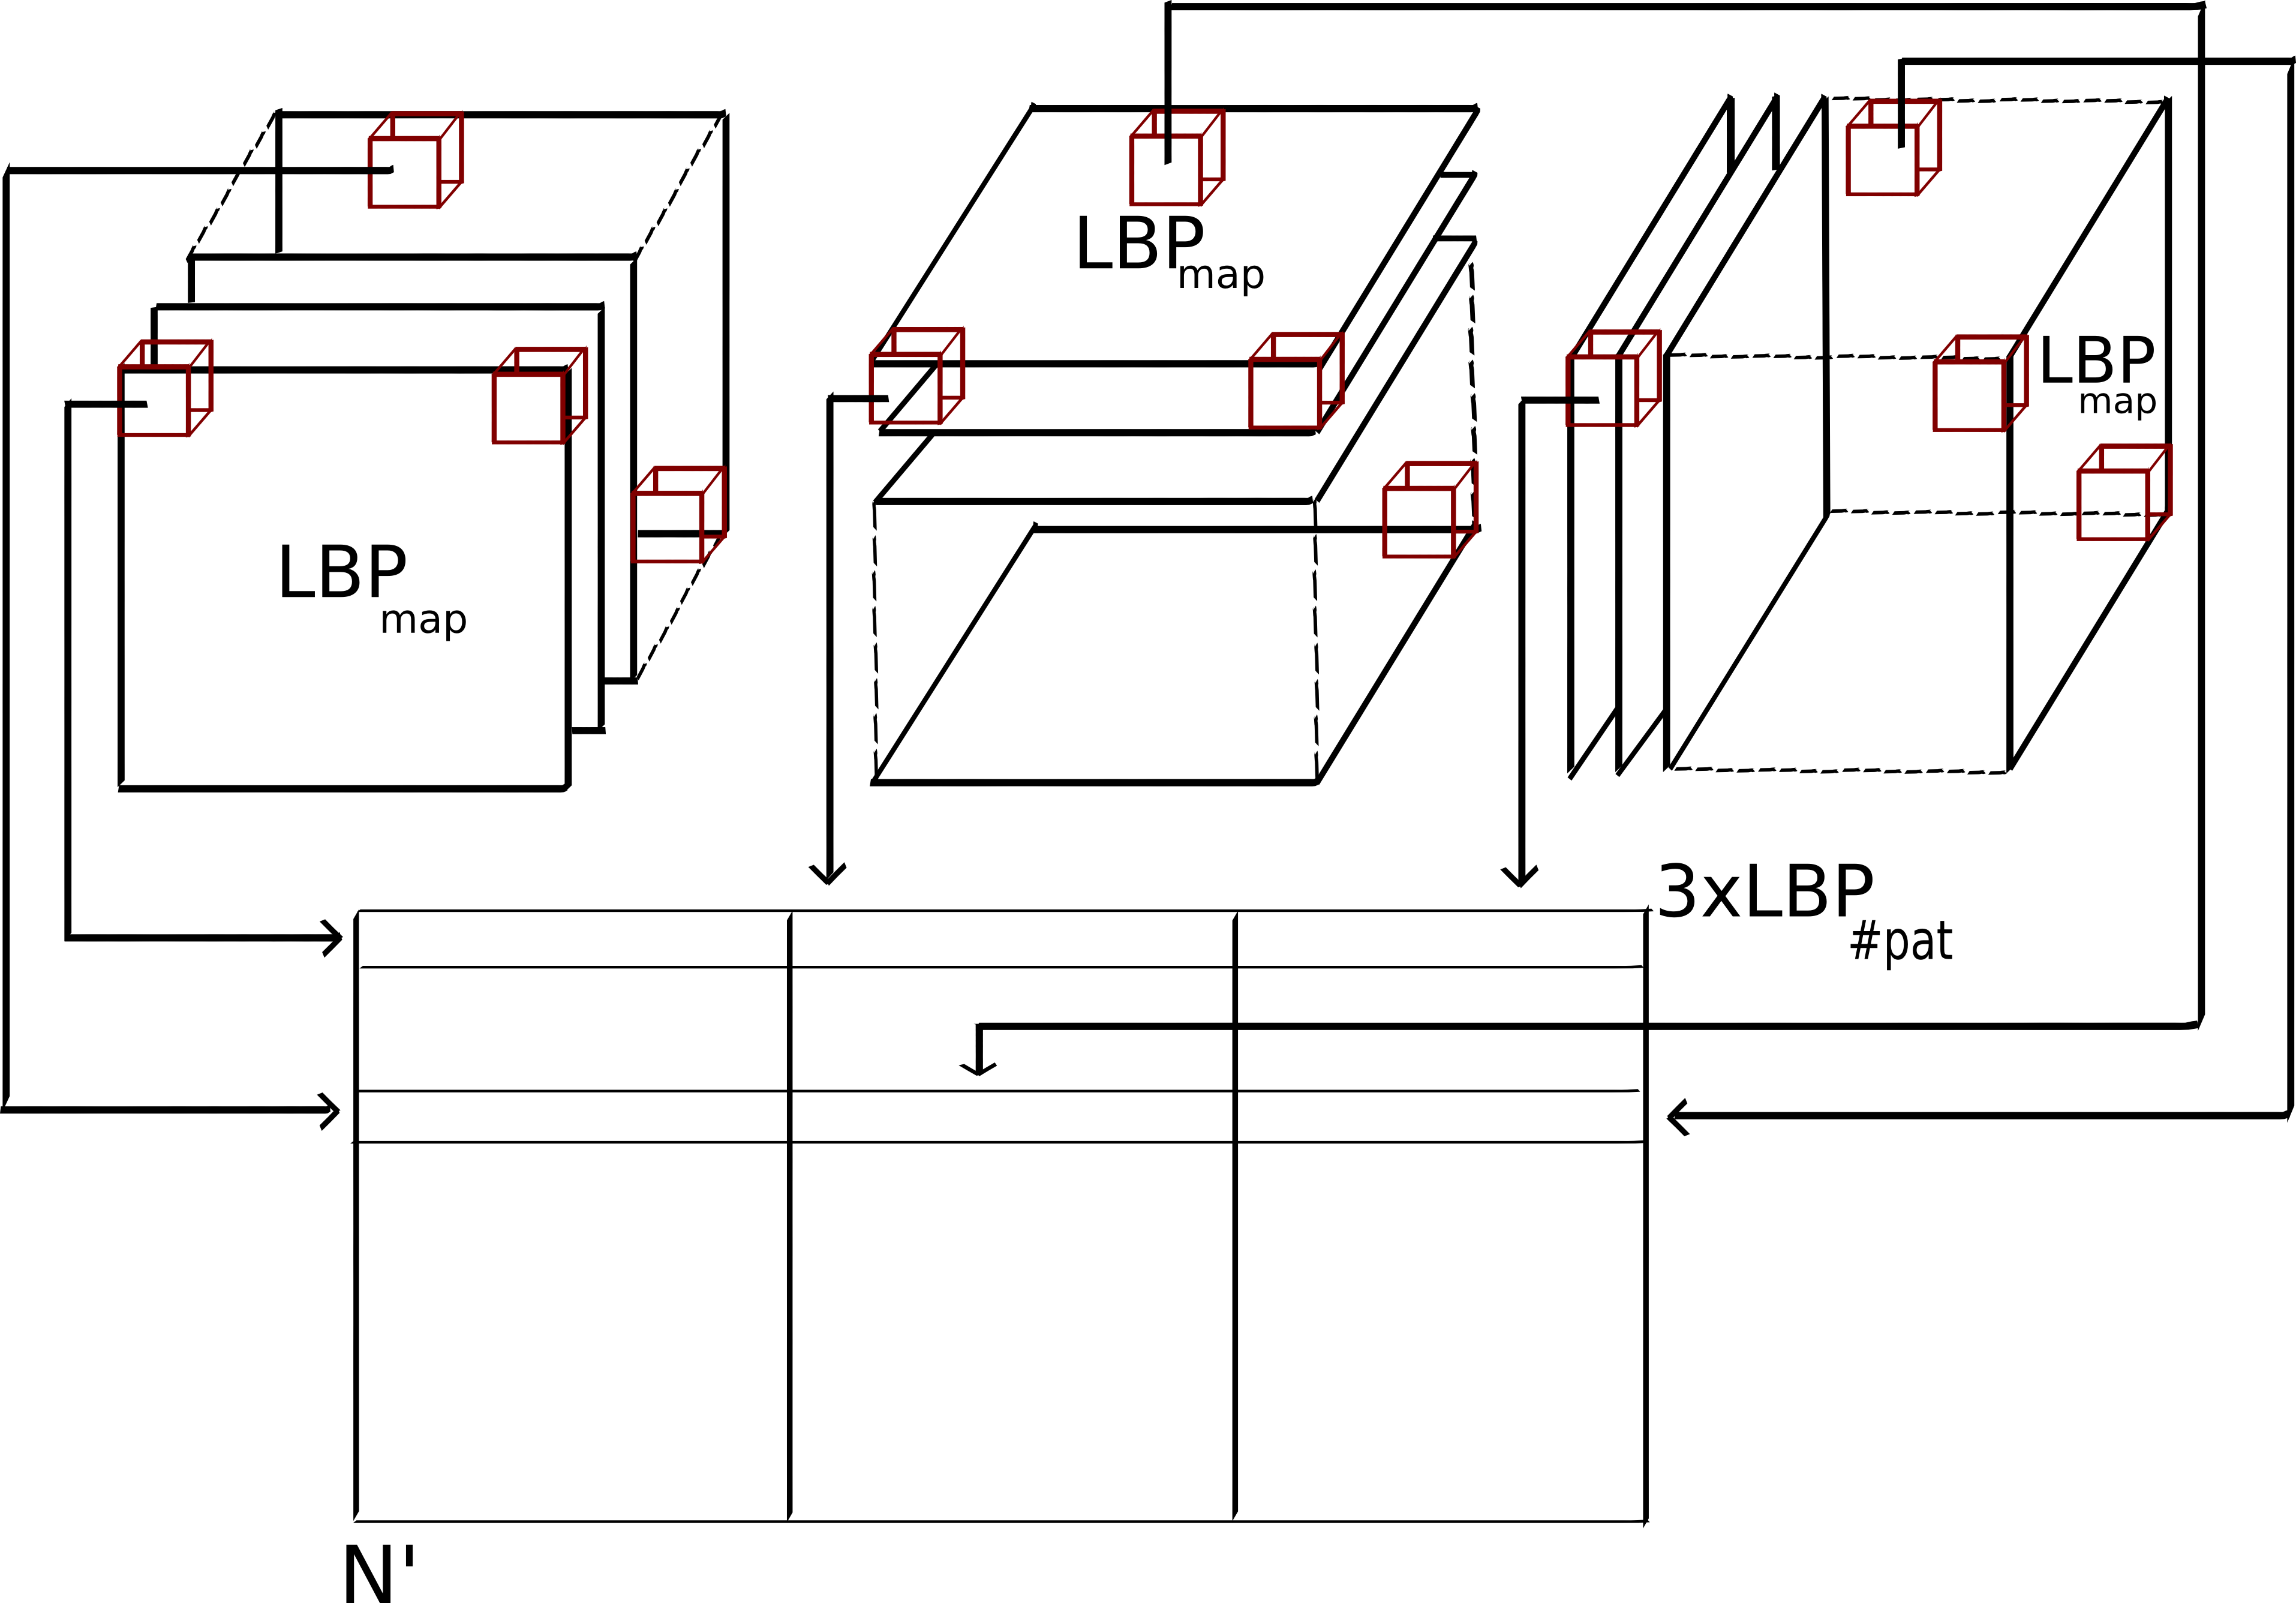
\includegraphics[width=0.48\linewidth]{local-lbptop.png}}
  \hspace*{\fill}
  \caption{Graphical representation of the feature extraction: (a) extraction of \ac{lbp} for global mapping - (b) extraction of \ac{lbptop} for global mapping - (c) extraction of \ac{lbp} for local mapping - (d) extraction of \ac{lbptop} for local mapping.}
  \label{fig:feaextimg}
\end{figure}

The size of the feature descriptor is summarized in Table~\ref{tab:descsize}.

\begin{description}
\item[\emph{Global}] mapping considers to extract the final descriptors from the 2D feature image for \ac{lbp} and 3D volume for \ac{lbptop}.
%mapping considers to extract the features from the 2D B-scans for \ac{lbp} and 3D volume for \ac{lbptop}.
Therefore, for a volume with $d$ slices, the \emph{global}-\ac{lbp} mapping will lead to the extraction of $d$ elements.
While the \emph{global}-\ac{lbptop} represents the whole volume as a single element.
The \emph{global} mapping for 2D images and 3D volume is shown in Fig.~\ref{subfig:glbp} and \ref{subfig:glbptop}.

\item[\emph{Local}] mapping considers to extract the final descriptors from a set of ($m \times m$) 2D patches for \ac{lbp} and a set of ($ m \times m \times m$) sub-volumes for \ac{lbptop}.
Given $N$ and $N'$ the total number of 2D patches and 3D sub-volumes respectively, the \emph{local}-\ac{lbp} approach provides $N \times d$ elements, while \emph{local}-\ac{lbptop} provides $N'$ elements.
%Here $N$ and $N'$ are the total number of elements per B-scane or the volume, respectively.
This mapping is illustrated in Fig.~\ref{subfig:llbp} and \ref{subfig:llbptop}.


\end{description}

%For the sake of clarification, the length of final descriptor for \emph{local} and \emph{global} mapping of both \ac{lbp} and \ac{lbptop} features with respect to the length of $\ac{lbp}_{hist}$ are listed in Table.~\ref{tab:tabmap}.
%
%\begin{table}[h]
%\caption{ Final length of descriptors of \ac{lbp} and \ac{lbptop} features, with respect to different mapping strategies and $\ac{lbp}_{hist}$ number of bins for various sampling point. Here $d$ is the number of B-scans per volumes and $N$ and $N'$ are the number of patches per B-scane and sub-volumes per volumes, respectively.}
%\centering
%\resizebox{1\linewidth}{!}{
%\scriptsize{
%\begin{tabular}{l ccc c ccc }
%\toprule
%Mapping & \multicolumn{3}{c}{\ac{lbp}} & & \multicolumn{3}{c}{\ac{lbptop}}\\
%\cmidrule(l){2-4} \cmidrule(l){6-8}
% & $\{8,1\}$ & $\{16,2\}$ & $\{24,3\}$ &  & $\{8,1\}$ & $\{16,2\}$ & $\{24,3\}$\\ 
% \midrule
%\emph{global} & $10 \times d $ & $ 18 \times d $ & $26 \times d$ & &  $ 3 \times 10 $ & $ 3 \times 18 $ & $3 \times 26$  \\
% & & & & & & & \\
%\emph{local} & $10 \times N \times d$ & $18 \times N \times d$ & $26 \times N \times d$ & & $3 \times 10 \times N' \times \frac{m}{d}$ & $3 \times 18 \times N'\times \frac{m}{d} $ & $3 \times 26 \times N'\times \frac{m}{d}$     \\
%\bottomrule
%\end{tabular}}
%}
%\label{tab:tabmap}
%\end{table}


\subsection{Feature representation}\label{subsec:fearep}

% Each \ac{oct} volume can be described by its texture and we employed two strategies.

% Sik: I would change this start by something like the following
%
% Our believe is that 'patology traits' present in the images can be captured bye means of thexture descriptors. In order to work with manage the descriptors, those should be represented in some fashion. Our framework incorporates two different manners of representing the volume descriptors.

%Depending of the textural feature (i.e., \ac{lbp} and \ac{lbptop}) and the mapping strategy (i.e., global or local), each volume can be represented into two different manners.

Two strategies are used to describe each \ac{oct} volume texture.

\begin{description}

\item[Low-level representation] The texture descriptor of an \ac{oct} volume is defined as the concatenation of the \ac{lbp} histograms with the \emph{global}-mapping.
The \ac{lbp} histograms are extracted from the previously computed \ac{lbp} maps (see Sect.\,\ref{subsec:feaext}).
Therefore, the \ac{lbptop} final descriptor is computed through the concatenation of the \ac{lbp} histograms of the three orthogonal planes with the final size of $3 \times LBP_{\#pat}$.
More precisely, an \ac{lbp} histogram is computed for each set of \ac{lbp} maps $(x$-$z)$ plane, $(x$-$y)$ plane, and $(y$-$z)$ plane, respectively.
Similarly, the \ac{lbp} descriptor is defined through concatenation of the \ac{lbp} histograms per each $(x$-$z)$ slice with the final size of $d \times LBP_{\#pat}$.

\item[High-level representation] The concatenation of histograms employed in the low-level representation in conjunction with either \emph{global}- or \emph{local}-mapping can lead to a high dimensional feature space.
For instance, \emph{local}-mapping results to a size of $N \times d \times LBP_{\#pat}$ for the final \ac{lbp} descriptor and $N' \times LBP_{\#pat}$ for the final \ac{lbptop} descriptor.
High-level representation simplifies this high dimensional feature space into a more discriminant lower space.
\ac{bow} approach is used for this purpose~\cite{Sivic2003}.
This model represents the features by creating a codebook or visual dictionary, from the set of low-level features.
The set of low-level features are clustered using \textit{k}-means to create the codebook with \textit{k} clusters or visual words.
After creating the codebook from the training set, the low-level descriptors are replaced by its closest word within the codebook.
The final descriptor is a histogram of size \textit{k} to represent the codebook occurrences for a given mapping.


%\Ac{pca} and \ac{bow} among other methods, are used for this purpose~\cite{Sivic2003}.
%Although \ac{pca} maps the data according to their variance, \ac{bow} models represent the features by creating a visual dictionary, or ``codebook'', from the set of low-level features.
%The set of low-level features is clustered using \textit{k}-means to create the codebook with \textit{k} defining the number of visual words.
%After creating the codebook, each of the training example is represented as a histogram of size \textit{k} obtained by calculating the frequency of occurrences of each of the \textit{k} words in the features extracted from the training example.

\end{description}

%\subsubsection{Low-level features} are extracted considering the whole volume using LBP and 3D-LBP descriptors.
% LBP is a discriminative rotation invariant feature descriptor proposed by Ojala et al. \cite{ojala2002multiresolution}.
% LBP descriptor encodes the intensity differences of a central pixel ($g_c$) with its neighboring pixels ($g_{p}$), within in a defined neighborhood of radius $R$. The differences are encoded in terms of binary patterns as in~Eq. \ref{Eq:LBP}:

% \begin{equation} \label{Eq:LBP}
% LBP_{P,R} = \sum_{p=0}^{P-1}s(g_{p} - g_{c})2^{p},
% \end{equation}
% where $s(a) = 1$ if $a \geq 0$, and $s(a)=0$ otherwise. $P$ is the number of sampling points in the circle of radius $R$.

% The binary patterns are calculated for each pixel in the given image and their histogram defines the final descriptor.
% The LBP histograms are computed for each slice of the volume and are concatenated into a single histogram. This forms the first low-level feature.
% The second low-level descriptor is defined in a similar manner as the first one. However principal component analysis (PCA) is applied to the concatenated histograms in order to reduce the dimension.

% For the third low-level descriptor, since the OCT data is a 3D volume, following the approach of Zhao \textit{et al}. \cite{zhao2007dynamic}, we extract 3D-LBP by considering three orthogonal planes, XY, XZ and YZ. Note that $X$, $Y$, and $Z$ are respectively the horizontal, vertical and depth direction of the OCT volume as shown in Figure~\ref{fig:oct_data}(a).
% LBP patterns are computed for each of the three planes, and the obtained three histograms are concatenated into a final 3D-LBP descriptor.



% \subsubsection{High-level features} - are extracted using bag of words (BoW) approach which is a feature representation technique based of creating a visual dictionary, or codebook, from a set of low-level features~\cite{Sivic2003}.
% To do so, the OCT images are divided into local patches and LBP histograms are computed for every local patch.
% This set of LBP histograms is then used to create a codebook using K-means clustering. If we define $K$ clusters in the feature space, then the visual dictionary will contain $K$ words each one being the center of one cluster.
% After creating the codebook, each of the training example is represented as a histogram of size $K$ obtained by calculating the frequency of occurrences of each of the $K$ words in the features extracted from the training example.
% Note that in the 2D case, each slice is divided into patches of size $N\times N$ and we extract 2D-LBP from each patch, while in the 3D case, the volume is divided into $N \times N \times N$ patches and 3D-LBP histograms are computed. In our experiments in Section 3, we set $N=7$, and vary the size of the codebook $K$ in the range $\{2, 4, 8, 16, 32, 64, 100 \}$.
% % \tikzstyle{block} = [rectangle, draw, fill=gray!20, text = black,
    text width=6em, text centered, rounded corners, minimum height=4em , minimum width = 6em]
    % \tikzstyle{line} = [draw, -latex']
  \tikzstyle{myarrow}=[->, thick]
    \tikzstyle{line}=[-, thick]
    \tikzstyle{block2} = [rectangle, draw, fill=white!20,
    text width=6em, text centered, rounded corners, minimum height=4em, minimum width = 6em]
    \tikzstyle{block3} = [rectangle, draw, fill=gray!20, text = black,
    text width=7em, text centered, rounded corners, minimum height=4em , minimum width = 7em]
\def\blockdist{1}
\def\edgedist{1.5}
  %%%% The Framework Sparse Coding 

\begin{figure}
 \begin{center}
   \begin{tikzpicture}[node distance = 1cm,scale=0.6, every node/.style={scale=0.6}]
%(FEx.east|- FEx.south)
    \node [block2] (input) {Training image};
    %\node [block, right of = input, node distance = 2.8cm](Seg){Segmentation}; 
    \node [block, right of=input,node distance = 2.8cm](De){Denoising};
    \node [block, right of=De,node distance = 2.8cm](FEx){Feature extraction};
    \path (FEx.east)+(+0.8,0) node (g) {};
    
    %%% Sparse Coding Block
    \node [block3, right of=g,node distance = 1.7cm](DL){Dictionary learning /k-means};
    \node [block3, below of=DL,node distance = 2.5cm](PR){Projection};
    \begin{pgfonlayer}{background}
      \path (DL.west |- DL.north)+(-0.4,-0.1+\blockdist) node (a) {};
      \path (PR.east |- PR.south)+(+0.4,-0.7) node (b) {};          
      \path[fill=gray!10,rounded corners, draw=gray!20, dashed] (a) rectangle (b);
    \end{pgfonlayer}
\path (DL.west |- DL.north)+(+1.2,-0.5+\blockdist) node (SP) {\textbf{Bag of Features}};
\path (PR.east |- PR.south)+(-1.3,-0.4+\blockdist) node (c){};
\path (PR.east)+(-3.15,0) node (d) {};

%%% Testing 
\node [block, below of=FEx, node distance = 2.5cm](FE2){Feature extraction};
\node [block, below of=De, node distance = 2.5cm](De2){Denoising};
% \node [block, below of=Seg, node distance = 2.5cm](Seg2){Segmentation}; 
\node [block2, below of=input, node distance = 2.5cm](TestImg){Testing image};

%%% 
\node [block, right of=PR, node distance = 3.6cm](Pool){Visual words histogram};
\path (Pool.east) + (0.3,0) node (f){}; 
\path (Pool.east) + (0.2,-0.1) node (f1){}; 

%%% Classification
\node [block, right of = Pool, node distance = 3.5cm] (Pre){Prediction}; 
    \node [block, above of = Pre, node distance = 2.5cm] (Learn){Learning}; 
    \begin{pgfonlayer}{background}
      \path (Learn.west |- Learn.north)+(-0.4,-0.1+\blockdist) node (h) {};
    \path (Pre.east |- Pre.south)+(+0.4,-0.7) node (i) {};          
    \path[fill=gray!10,rounded corners, draw=gray!20, dashed] (h) rectangle (i);
\end{pgfonlayer}
\path (Learn.west |- Learn.north)+(+1.1,-0.5+\blockdist) node (Clas) {\textbf{Classification}};
\path (Pre.east |- Pre.south)+(-1.3,-0.4+\blockdist) node (j){};
\path (f1.north)+(0, 2.5) node (k) {};
\path (Pre.east) + (1.2,0) node (k1) {P(..)}; 

    % Draw edges
    \draw [line] (input) -- (De) -- (FEx); 
    \draw [myarrow] (FEx)-- (DL);
    \draw [myarrow] (DL) -- (PR) ; 
    \draw [line] (TestImg) -- (De2) -- (FE2); 
    \draw [myarrow] (FE2) -- (PR) ;
    \draw [line] (PR) -- (Pool); 
    \draw [myarrow] (Pool) -- (Pre); 
    \draw [line] (f1.north) -- + (0,2.5)(k.south); 
    \draw [myarrow] (k.south)+ (0,0.1)  -- (Learn.west); 
    \draw [myarrow] (Pre) -- (k1);

    \end{tikzpicture}
    \end{center}
    

\caption{Bag of features framework} 
\label{fig:BoF-framework}

\end{figure}

\subsection{Classification}\label{subsec:cls}
% Classification is a supervised learning method which intends to find a mapping $f(.)$ which relates a set of input $x$ to a set of categorical outputs $y$.
% The learning is comprehended using a training set, which contains a set of $N$ samples with their associated labels~\cite{murphy2012machine}.

Classification corresponds to the mapping of a set of inputs $\mathbf{x}$ into a set of categorical outputs $\mathbf{y}$ using a linear or non-linear function $f(\cdot)$.
In supervised learning methods, this function is defined by providing a training set of $N$ samples $\mathbf{x}_{tr}$ with their associated labels $\mathbf{y}_{tr}$.
In order to make a comparative study, five different classifiers are used: (i) $k$-\acf{nn}, (ii) \acf{lr}~\cite{cox1958regression}, (iii) \acf{rf}~\cite{breiman2001random}, (iv) \acf{gb}~\cite{friedman2002stochastic, lemaitre2015boosting}, and (v) \acf{svm}~\cite{vapnik1963generalized, aizerman1964}.
%In the remainder of this section, we briefly summarize the supervised classification methods used in the experiments.
Details regarding the parameters used in our experiments are provided in Sect.\,\ref{sec:exp}.

% \begin{description}

% \item[$k$-\acf{nn}] is a non-parametric classification method in which an unlabeled feature vector $x$ is assigned to the majority class of its $k$ nearest-neighbors from the training set.
% To avoid a tie case, the parameter $k$ is set to an odd number.

% \item[\acf{lr}] is a linear classifier which uses the logistic function to estimate the probability of $x$ to belong to a particular class $c_i$~\cite{cox1958regression}.
% Thus, the posterior probability is expressed as:
% \begin{equation} \label{eq:ppc1lr}
% p(c_{i}|x) = \frac{1}{1+\exp(-w^{T}x)}
% \end{equation}
% \noindent where $w$ is a vector of the regression parameters to obtain a linear combination of the input feature vector $x$.
% The vector $w$ can be inferred by finding the maximum likelihood estimates via optimization methods such as quasi-Newton method~\cite{byrd1994representations}.
% Once the vector $w$ is found, an unlabeled feature vector is assigned to the class which maximizes the posterior probability.
% % \begin{equation}
% % C(x) =  \text{arg}\max\limits_{k} p(C = k| x)
% % \end{equation}

% \item[\acf{rf}] is an ensemble of decision trees~\cite{breiman2001random} which generalizes the classification process by applying two types of randomization: at the tree level, each tree is fed by a bootstrap made of $S'$ samples which are built from the original data of size $S$ such that  $S=S'$, and at the node level, a subset of feature dimensions $m$ is randomly selected from the original dimension $M$ such that $m << M$.
% The trees in \ac{rf} are grown to their maximum length without any pruning.
% In the testing stage, each tree in the ensemble casts a unit vote in the final prediction and the final prediction is based on combination of all the votes.
% % is an ensemble of decision trees~\cite{breiman2001random}.
% % The ensemble uses each tree to predict an output and finalizes the ultimate prediction by aggregating the outputs of all tress.
% % This classifier learns the data by training multiple decision trees on bootstrap samples of the original data.
% % Each bootstrap of $D$ dimension is used for training one decision tree and at each node, the best split among randomly ($d << D$) selected subset of descriptors is chosen.
% % Each tree is grown to its maximum length without any pruning.
% % In the prediction stage a sample is voted by each tree and it is labeled by considering the majority of the votes.

% \item[\acf{gb}] is a reformulation of \ac{adb}~\cite{friedman2002stochastic} in which the problem of finding an ensemble of real-valued weak learners is tackled as a numerical optimization~\cite{lemaitre2015boosting}.
% A strong learner is built by iteratively finding the best pair of real-valued weak learner function and its corresponding weight which minimizes a given differentiable loss function.
% Common choice for weak learners is decision stumps or regression trees while the loss function is generally an exponential or logarithmic loss~\cite{becker2013supervised}, minimized via gradient descent or quadratic approximation.

% \item[\acf{svm}] is a sparse kernel classification method which aims at finding the best linear hyperplane which separates two classes by maximizing the margin between them~\cite{vapnik1963generalized}.
% \ac{svm} becomes a non-linear classifier by using the kernel trick~\cite{aizerman1964} which consists in replacing each inner product by a non-linear kernel function such as \ac{rbf} or polynomial kernels.
% % Maximizing the margin is equivalent to minimizing the norm of the normal vector of the hyperplane:
% % \begin{equation}
% % \min\limits_{\mathbf{w}, \omega_{0}} \frac{1}{2} \Vert \mathbf{w}\Vert^{2} \qquad \text{s.t. } \quad  y_{i}(\mathbf{w}^{T}\mathbf{x_{i}} + \omega_{0}) \geq 1, i = 1: N
% % \label{eq:svmsm}
% % \end{equation}
% % \noindent This constraint intends to force all the point to be in the correct side of the decision boundary (hyperplane) with a minimum distance of 1.
% % This assumption is only valid if the data is linearly separable.
% % Thus for general cases a slack variable $\xi_{i} \geq 0 $ is introduced, which is $\xi_{i} = 0 $, if the points are on/or inside the correct margin boundary, is $0 < \xi_{i} \leq 1 $ if the points are inside the margin but in the correct side of the decision boundary and otherwise if they lie in the wrong side of decision boundary is $\xi_{i} > 1 $.
% % This assumption introduces the \textit{soft margin constraints}.
% % Therefore the optimization problem of \ac{svm} classifier is presented by:

% % \begin{align}
% %  & \min\limits_{\mathbf{w},\omega_{0}, \mathbf{\xi}} \frac{1}{2} \Vert \mathbf{w} \Vert^{2} + C \sum\limits_{i = 1}^{N} \xi_{i} \nonumber \\
% % \text{s.t. } & \quad \xi_{i} \geq 0, \quad y_{i}(x_{i}^{T}\mathbf{w} + \omega_{0}) \geq 1 - \xi_{i}, i = 1:N
% % \label{eq:svmop}
% % \end{align}
% % In Eq.~\ref{eq:svmop}, the $\sum_{i} \xi_{i}$ term, describes the upper bound on the number of misclassified points and $C$ is the regularization parameter that controls the tolerance of the classifiers on the number of errors~\cite{murphy2012machine}. \\

% \end{description}


% Random Forest


%%% Local Variables:
%%% mode: latex
%%% TeX-master: "../../main.tex"
%%% End:
